% 1989 年上海卷第一题第 6 小题：长方体 ABCD-A'B'C'D' 示意图；透视比例不代表题设尺寸
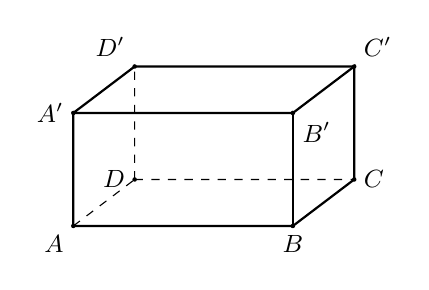
\begin{tikzpicture}[scale=0.82,>=stealth,font=\small]
  \coordinate (A) at (0,0);
  \coordinate (B) at (3.4,0);
  \coordinate (C) at (4.35,0.72);
  \coordinate (D) at (0.95,0.72);
  \coordinate (Ap) at (0,1.75);
  \coordinate (Bp) at (3.4,1.75);
  \coordinate (Cp) at (4.35,2.47);
  \coordinate (Dp) at (0.95,2.47);
  \draw[thick] (A)--(B)--(C)--(Cp)--(Bp)--(Ap)--cycle;
  \draw[thick] (Ap)--(Dp)--(Cp);
  \draw[thick] (A)--(Ap) (B)--(Bp);
  \draw[dashed] (A)--(D) (D)--(C) (D)--(Dp);
  \fill (A) circle (1pt) node[below left] {$A$};
  \fill (B) circle (1pt) node[below] {$B$};
  \fill (C) circle (1pt) node[right] {$C$};
  \fill (D) circle (1pt) node[left] {$D$};
  \fill (Ap) circle (1pt) node[left] {$A'$};
  \fill (Bp) circle (1pt) node[below right] {$B'$};
  \fill (Cp) circle (1pt) node[above right] {$C'$};
  \fill (Dp) circle (1pt) node[above left] {$D'$};
\end{tikzpicture}
